\documentclass[main.tex]{subfiles}
\begin{document}

\href{https://www2.seas.gwu.edu/~simhaweb/quantum/modules/review/comp-review/comp-review.html}{Computing Review}

\subsection{Binary numbers}

Consider a decimal example such as the number 243: $2 \times 10^{2}+4 \times 10^{1}+3 \times 10^{0}$. Here, the terminology is that 10 is the base of the number system. The lowest power (0) occurs at the rightmost position, with each successive digit going leftwards, representing a multiple of a higher power of the base. There needs to be a separate symbol for each number less than the base, in our case: $0,1, \ldots, 9$. One can take this a step further and add decimals to the right of the $10^{\circ}$ position with a "marker" (decimal point) to help readability For example, 243.51: $2 \times 10^{2}+4 \times 10^{1}+3 \times 10^{0}+5 \times 10^{-1}+1 \times 10^{-2}$. The same positional principles apply to binary numbers: Since we're using powers of 2 , there are only 2 symbols $(0$ and 1$)$. For example, the number 1101: $1 \times 2^{3}+1 \times 2^{2}+0 \times 2^{1}+1 \times 2^{0}=13$ (in decimal). Each digit is called a bit. The above number is a 4-bit binary number. An 8-digit binary number is called a byte. Positional addition in binary works as it does in decimal as shown in Figure \ref{fig:01_addition}. We will occassionally see binary numbers represented by the bits $x_{n-1} x_{n-2} \ldots x_{0}$, where each $x_{i} \in\{0,1\}$. In this case, the actual value of the number is: $\sum_{i=0}^{n-1} x_{i} 2^{i}$.\\

\begin{figure}
    \centering
    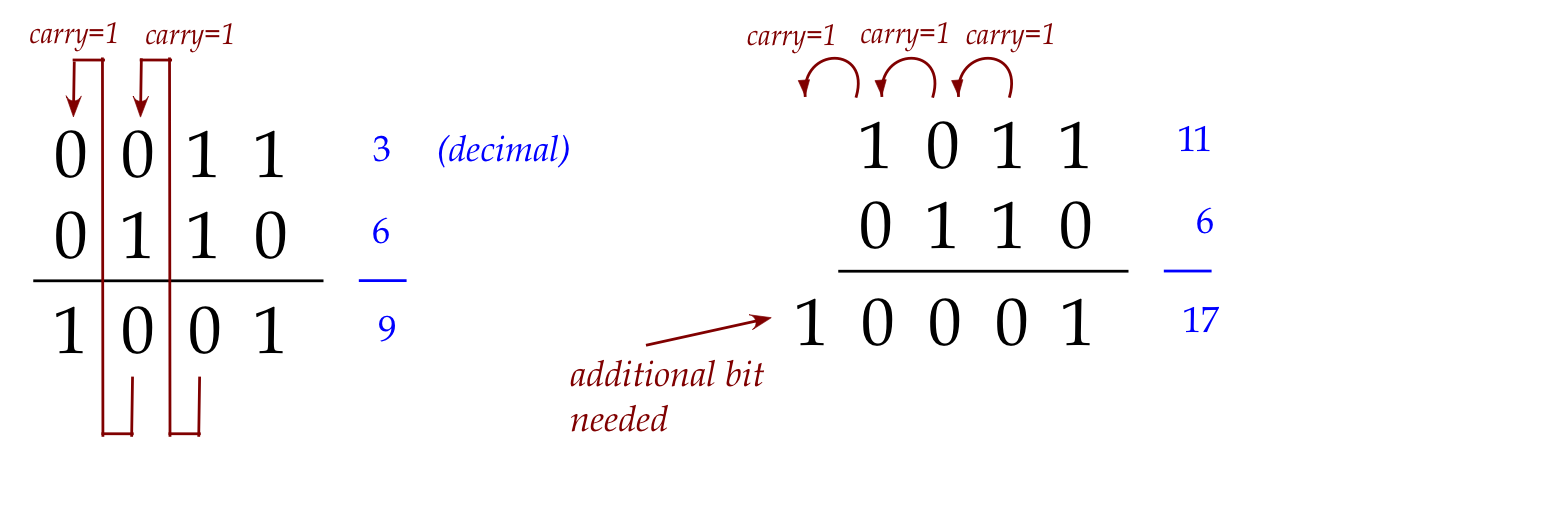
\includegraphics[width=5in]{notes/figs/n03/01_addition.png}
    \caption{Binary Additions}
    \label{fig:01_addition}
\end{figure}

Why is the binary representation of numbers important? It isn't because they're convenient to reason with. It's because the physical devices we use to store and manipulate numbers are binary in nature. It's a limitation of our ability to manufacture devices. In hardware, it's easy to create devices that are two state: either "on" or "off". Each such storage device that holds one binary digit is also called a bit. As we will see later, a qubit or quantum bit is quite different. A single qubit will store a $2 \mathrm{D}$ complex vector.

\subsection{Boolean functions}

Let us, for a moment, look at a 2-input 1-output real-variable function like we've seen before, for example: $f\left(x_{1}, x_{2}\right)=3 x_{1}+x_{2}^{2}$. We can think of the function as a box that takes in two real numbers, "does something" with those numbers and outputs a real number as result. For example, $f(1.5,3)=3 \times 1.5+3^{2}=13.5$, as shown in Figure \ref{fig:02_func-example}. While the inputs and output are real numbers, the notion of "doing something" with inputs to produce an output is more general. Also, let's think of a variable as holding or representing a real number as a value.\\

\begin{figure}
    \centering
    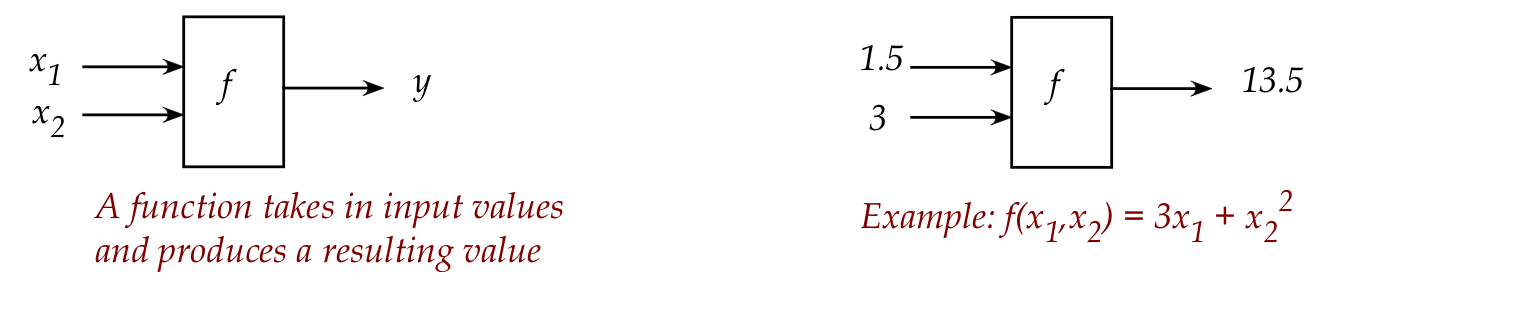
\includegraphics[width=5in]{notes/figs/n03/02_func-example.png}
    \caption{Function Input and Resulting Value}
    \label{fig:02_func-example}
\end{figure}

A Boolean function: Suppose we consider Boolean variables: Just as a real variable holds or represents a real number, a Boolean variable holds just one of two values: True or False. For convenience we'll use T for True and F for False. Then, a Boolean function, say of two variables, takes in two Boolean values and outputs a Boolean value. Unlike real-valued functions, which can be of infinite varieties, Boolean functions are limited in what they can do. For example, consider a 1-input, 1-output Boolean function $f(x)$. The input can only be $\mathrm{T}$ or $\mathrm{F}$. The output can only be T or F. Here's one possible function
$f_{1}(T)=T$, $f_{1}(F)=F$, here's another $f_{2}(T)=F$, $f_{2}(F)=T$ and two more:
$f_{3}(T) =T$, $f_{4}(T) =F$, $f_{3}(F) =T$, $f_{4}(F) =F$. There aren't any more - we have enumerated all possible 1-input 1-output Boolean functions.\\

Truth tables and well-known Boolean functions: A truth table is a convenient way to specify Boolean functions. For example, consider this 2-input 1-output Boolean function shown in Figure \ref{fig:03_truthtable}. Observe: Because there are only a finite number of input possibilities, a truth table lists all of them. For each input possibility, the output is explicitly stated. The above Boolean function is called the AND-function, sometimes written as the binary operator $\wedge$ between the variables as $x_{1} \wedge x_{2}$. The intuition is that the output is True only when both inputs are True. It is common to use 0 for False and 1 for True, as shown on the right above. Because of this, the multiplication "as numbers" of $x_{1} x_{2}$ produces the same result as AND. However, when both are 1, we get $x_{1}+x_{2}=2$, a non-Boolean value for addition. To address this problem, we use $x_{1}+_{2} x_{2}=1$, where the symbol $+_{2}$ means "add, then take the remainder after integer-dividing by 2 ".\\

\begin{figure}
    \centering
    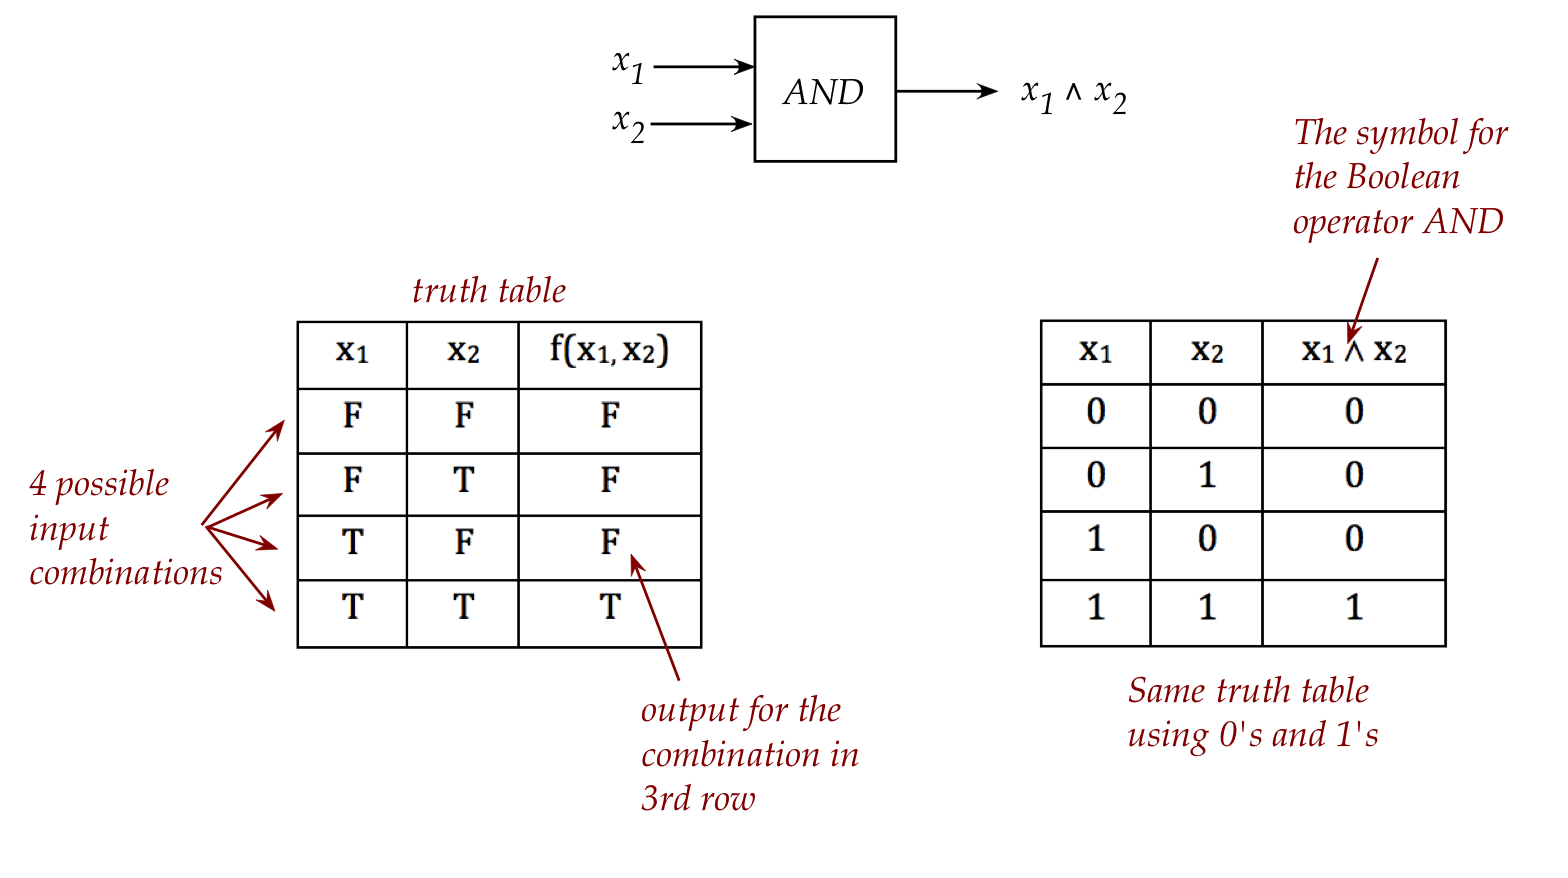
\includegraphics[width=5in]{notes/figs/n03/03_truthtable.png}
    \caption{Truth Table}
    \label{fig:03_truthtable}
\end{figure}

The other major 2-input 1-output function is the Boolean OR operation, written as $x_{1} \vee x_{2}$ with truth table shown in Figure \ref{fig:04_truthtable_OR}. Additionally we have the NAND truth table, and for quantum computing, the XOR (exclusive OR) truth table shown in Figure \ref{fig:05_truthtable_NAND_and_XOR}. The way to remember this function: the output is 1 when the two inputs are different. Symbolically, this is written as $x_{1} \oplus x_{2}$ The only 1-input 1-output function of real use is the NOT function that "flips" the value as shown in Figure \ref{fig:06_truthtable_NOT}. Figure \ref{fig:07_truthtable_three_values} is a 3-input 1-output example. Notice how the truth table has doubled in size to account for all possible 3-input combinations.

\begin{figure}
    \centering
    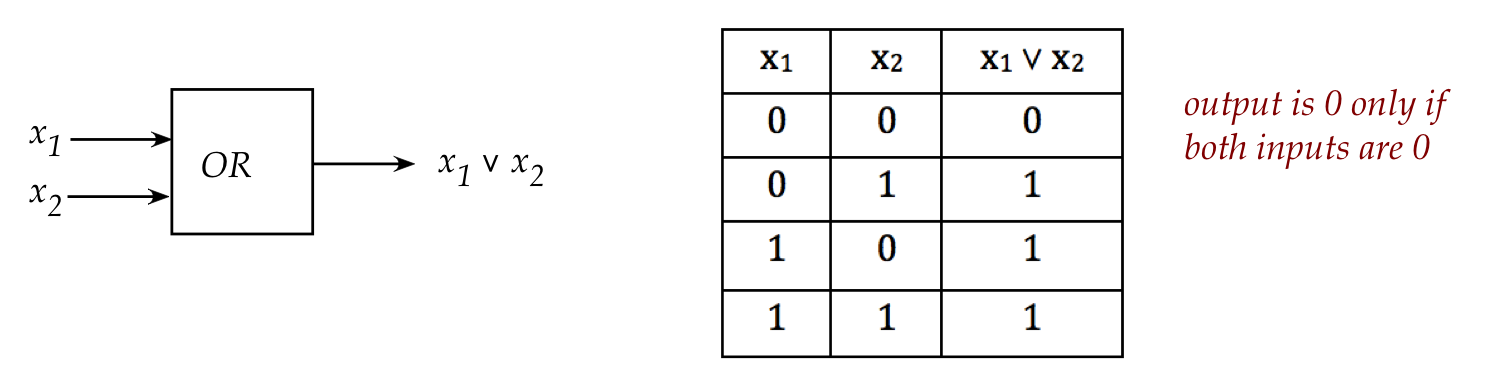
\includegraphics[width=5in]{notes/figs/n03/04_truthtable_OR.png}
    \caption{OR Truth Table}
    \label{fig:04_truthtable_OR}
\end{figure}

\begin{figure}
    \centering
    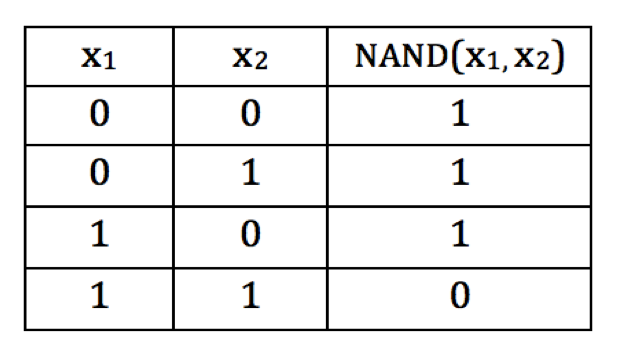
\includegraphics[width=2in]{notes/figs/n03/05_truthtable_NAND.png}
    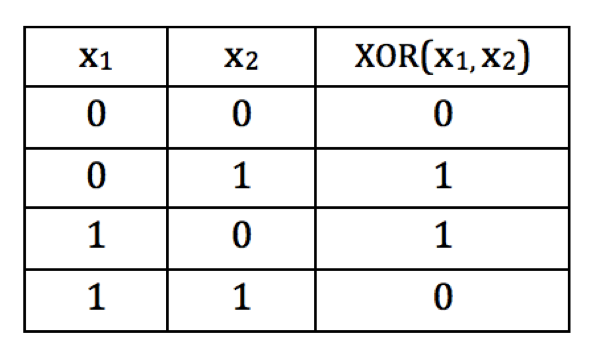
\includegraphics[width=2in]{notes/figs/n03/06_truthtable_XOR.png}
    \caption{NAND and XOR Truth Table}
    \label{fig:05_truthtable_NAND_and_XOR}
\end{figure}

\begin{figure}
    \centering
    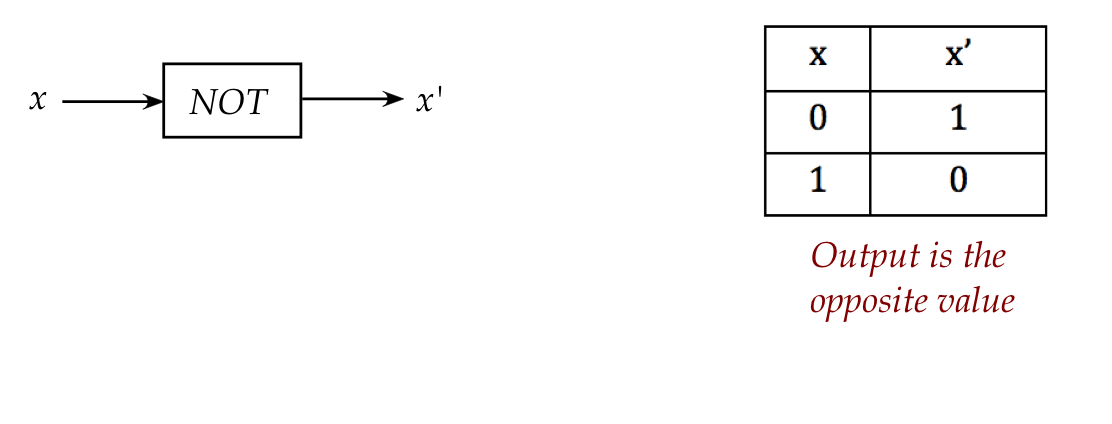
\includegraphics[width=4in]{notes/figs/n03/07_truthtable_NOT.png}
    \caption{Not Truth Table}
    \label{fig:06_truthtable_NOT}
\end{figure}

\begin{figure}
    \centering
    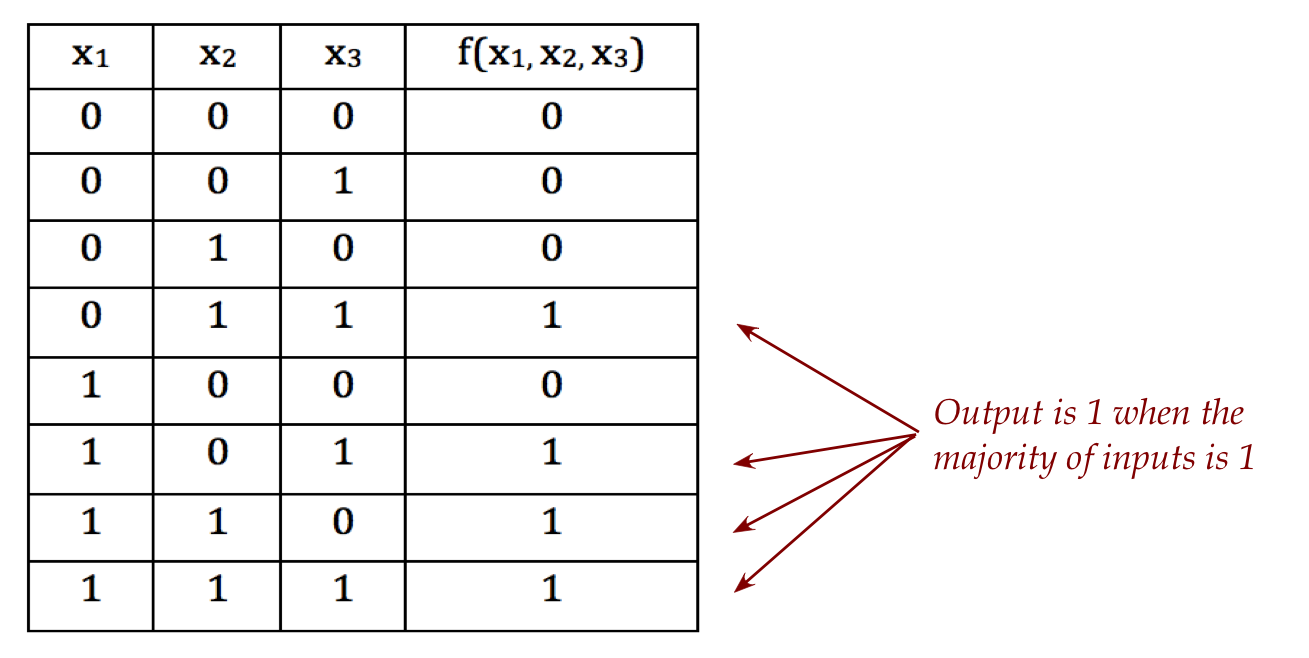
\includegraphics[width=4in]{notes/figs/n03/08_truthtable_three_values.png}
    \caption{Three Value Truth Table}
    \label{fig:07_truthtable_three_values}
\end{figure}

\subsection{Boolean algebra}

Just as ordinary numeric variables can be combined with numeric operators in expressions, so can Boolean variables and operators. For example: $f\left(x_{1}, x_{2}, x_{3}\right)=\left(x_{1}^{\prime} \wedge x_{2}\right) \vee\left(x_{1} \wedge x_{2}\right) \vee\left(x_{2} \wedge x_{3}^{\prime}\right)$ and just like in numeric expressions, there are all kinds of simplification rules (distributivity, associativity and so on) to help simplify, for example: $f\left(x_{1}, x_{2}, x_{3}\right) = \left(x_{1}^{\prime} \wedge x_{2}\right) \vee\left(x_{1} \wedge x_{2}\right) \vee\left(x_{2} \wedge x_{3}^{\prime}\right) = \left(\left(x_{1}^{\prime} \vee x_{1}\right) \wedge x_{2}\right) \vee\left(x_{2} \wedge x_{3}^{\prime}\right) = x_{2} \vee\left(x_{2} \wedge x_{3}^{\prime}\right)$. Sometimes, we repurpose numeric addition and multiplication conventions and write
$f\left(x_{1}, x_{2}, x_{3}\right) &=x_{1}^{\prime} x_{2}+x_{1} x_{2}+x_{2} x_{3}^{\prime} =\left(x_{1}^{\prime}+x_{1}\right) x_{2}+x_{2} x_{3}^{\prime} = x_{2}+x_{2} x_{3}$ Here, it's understood that ' $+$ ' refers to Boolean OR. What do we know about such simplifications? It turns out to be an important problem in the design of hardware, where understandably, one wants as few operations as possible. Finding an optimized function (minimum number of operations) is a challenging (and interesting) problem. There's a simple way to build an expression from truth table as shown in Figure \ref{fig:08_truthtable_build}.\\

\begin{figure}
    \centering
    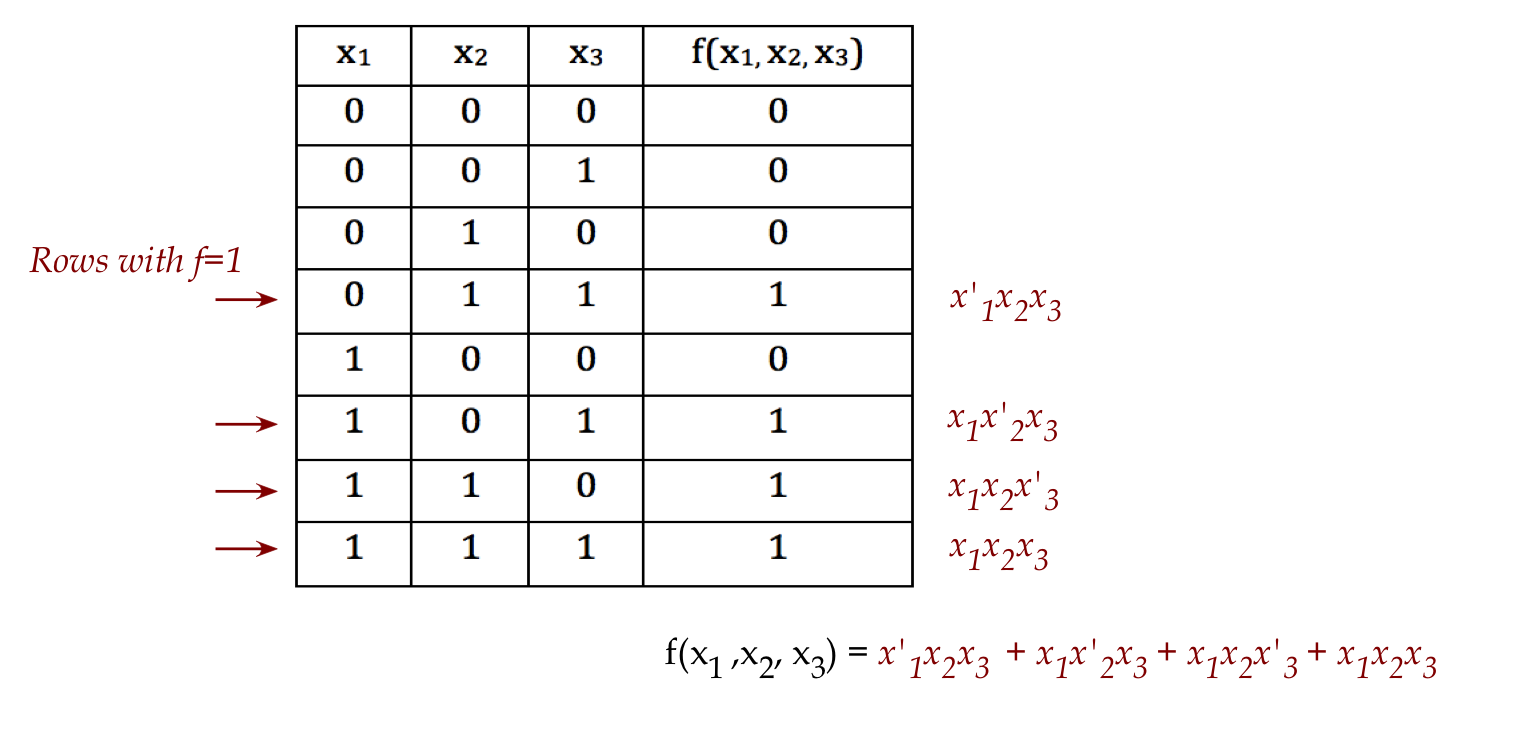
\includegraphics[width=5in]{notes/figs/n03/09_circuit5.png}
    \caption{Build Expression from Truth Table}
    \label{fig:08_truthtable_build}
\end{figure}

Identify the rows where the end output is 1. To get a particular row's outcome to occur, the variable values have to match the row's input specification exactly. Then, the output will be 1 if the inputs match any of these rows. "Any of these $\mathrm{f}=1$ rows" is expressed by the OR of the individual rows. This approach provides a systematic way to build an expression for a desired Boolean function: Build a truth table for the function. Write out the expression resulting from OR-ing the $f=1$ rows. Optimize to simplify the expression. But what do we do with a Boolean expression had XOR and NAND operators? This raises an important concept (for quantum computing): universality.\\

Universal Boolean operators: We now know that XOR and NAND can be written entirely in terms of AND/OR/NOT via the truthtable-to-expression approach shown in Figure \ref{fig:10_XOR_NAND_truthtable_expression}. The set of gates $\{AND, OR, NOT\}$ is universal: We can turn any Boolean function into a truth table and convert into an expression just using AND/OR/NOT gates. What is less obvious is that there are other universal sets. Perhaps surprisingly, just the NAND gate by itself is universal! The question of universality for Boolean gates now seems addressed with AND/OR/NOT. However, the same question (of universality) for quantum gates is not so straightforward, as we'll see. Lastly, to round out our quick overview of Boolean algebra, let's describe the problem of satisfiability: Consider an equation like $2 x_{1}+3 x_{1}^{2}-x_{2}=13$. This happens to have multiple solutions, for example $x_{1}=2, x_{2}=3$ or $x_{1}=1, x_{2}=-8$. Notice that one variable appears twice. In general a variable can occur multiple times. The general form of an equation is to have an expression with variables on the left, and a constant (a value) on the right. We can write Boolean equations too, for example, $\left(x_{1}^{\prime} \wedge x_{2}\right) \vee\left(x_{1}^{\prime} \wedge x_{3}\right)=T$ and ask if there are solutions. Broadly, this is called the satisfiability problem: given a boolean equation, can one find True/False values for the variables to make the equation hold? Notice that we can omit the right side and just ask whether the expression on the left can be made True? It is common to restrict the type of Boolean expression to be in Conjunctive Normal Form (CNF): For example:
$\left(x_{1}^{\prime} \vee x_{2} \vee x_{4}^{\prime}\right) \wedge\left(x_{2} \vee x_{3}^{\prime}\right) \wedge\left(x_{1} \vee x_{2}^{\prime} \vee x_{3}\right) \wedge\left(x_{1} \vee x_{2} \vee x_{3}\right)$. In this form, there are a bunch of clauses in parentheses (four clauses above). The only operators allowed inside a clause are $\mathrm{O}$ and complement. The complement is only applied to individual variables. It turns out that any Boolean expression can be algebraically manipulated into this form, so it's not restrictive. When the number of variables present in each clause is restricted, for example, to at most $K$ variables, the problem is called K-satisfiability. In the above example, the biggest clause has 3 variables, so it's an instance of a 3-Satisfiability problem. Often, we use the shorter term K-SAT. The satisfiability problem is one of the most important problems in computer science: No efficient algorithm is known for this problem. If an efficient algorithm were to be found, it can be shown that the algorithm can be used to efficiently solve thousands of other important problems. In that sense, satisfiability is (strangely) a universal problem. We will later see how quantum computing offers some hope of finding solutions to satisfiability.

\begin{figure}
    \centering
    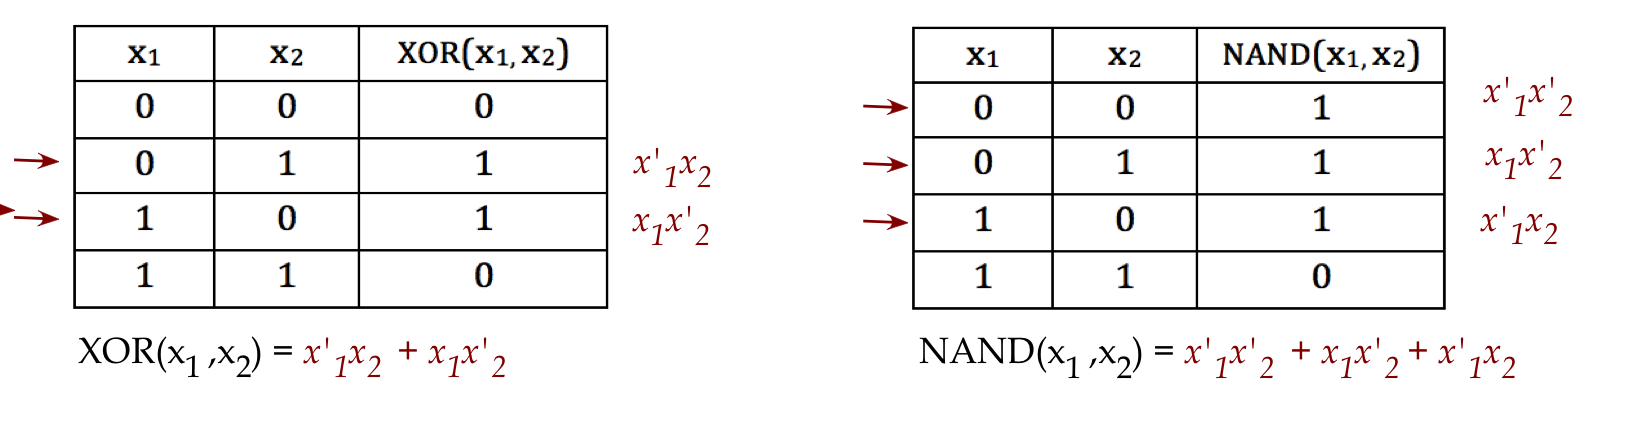
\includegraphics[width=5in]{notes/figs/n03/10_circuit6.png}
    \caption{XOR and NAND Truth Table Expressions}
    \label{fig:10_XOR_NAND_truthtable_expression}
\end{figure}

\subsection{Boolean circuits}

Let's return to the OR function above and imagine how this might be implemented physically with electronic circuitry as shown in Figure \ref{fig:11_OR_electronic_circuitry}. How to think of this: Think of the $\mathrm{O}$ box as some circuitry that is set up to receive electronic pulses on the input wires, and to issue electronic pulses on the output wire. When the top input wire has nothing (interpreted as 0 ), and the bottom one has an actual pulse (high enough voltage), then the $OR$ circuit "does its thing", which is to soon after produce a burst of electricity (pulse) on the output wire. Thus, a little more abstractly, one can think of 0 's and 1 's "flowing" through a circuit at discrete time steps. Consider \ref{fig:12_AND_NOT_electronic_circuitry}. Here we see that one can arrange these functional devices in sequence to produce a result. In a circuit context, the boxes that perform the basic Boolean operations like AND, OR, are called gates. We can reason about such combinations of Boolean gates in Figure \ref{fig:13_AND_NOT_electronic_circuitry_truthtable}. By systematically trying all input combinations, we can describe the output for each. Recognize the truth table on the right? Inputs can be staggered in, as in Figure \ref{fig:14_AND_NOT_OR_electronic_circuitry}. Note: the "pulse" of electricity for $x_3$ would have to be held long enough or timed to give enough time for $y$ to be created.\\

\begin{figure}
    \centering
    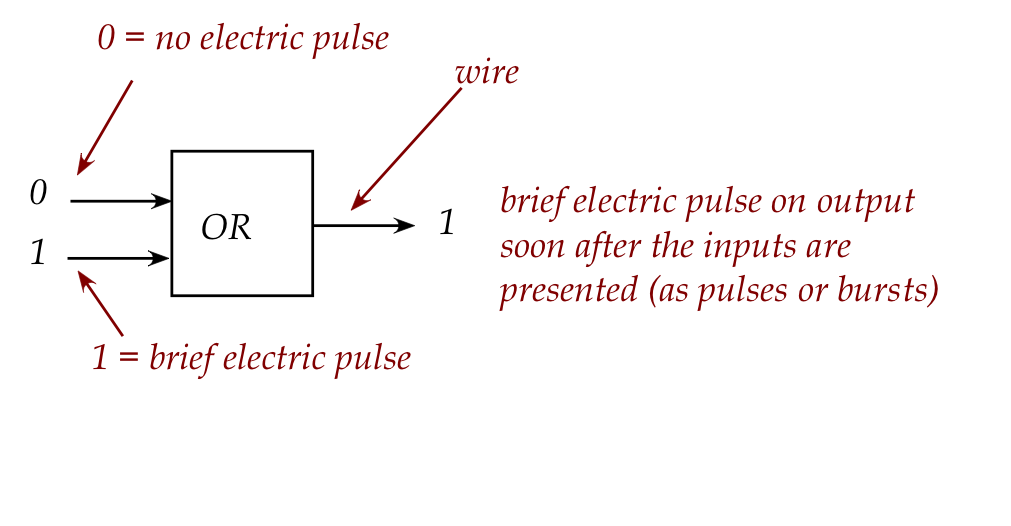
\includegraphics[width=5in]{notes/figs/n03/11_circuit1.png}
    \caption{OR Electronic Circuitry}
    \label{fig:11_OR_electronic_circuitry}
\end{figure}

\begin{figure}
    \centering
    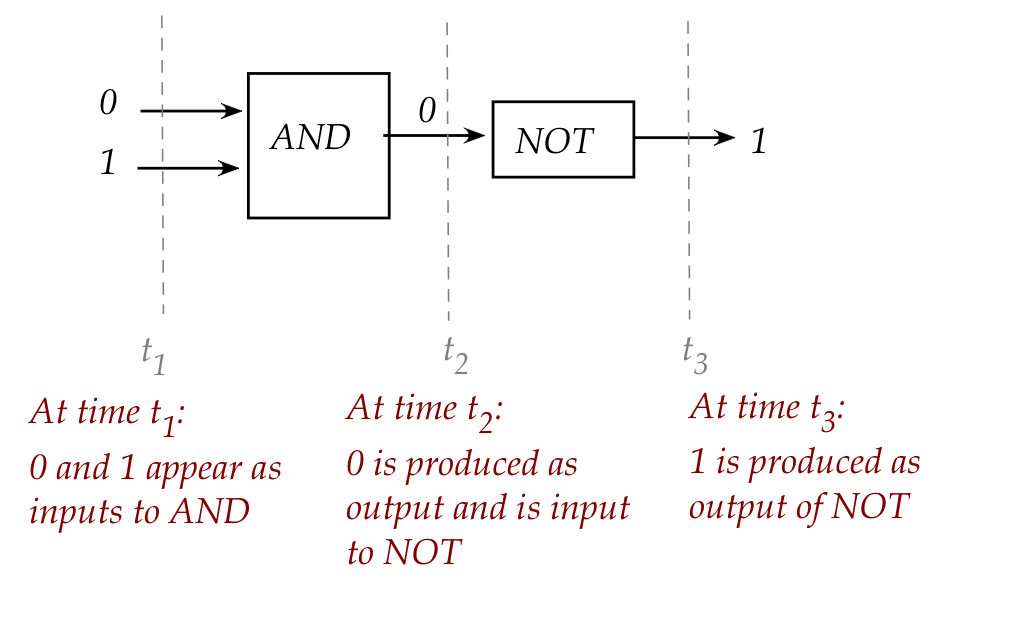
\includegraphics[width=5in]{notes/figs/n03/12_circuit2.png}
    \caption{AND NOT Electronic Circuitry}
    \label{fig:12_AND_NOT_electronic_circuitry}
\end{figure}

\begin{figure}
    \centering
    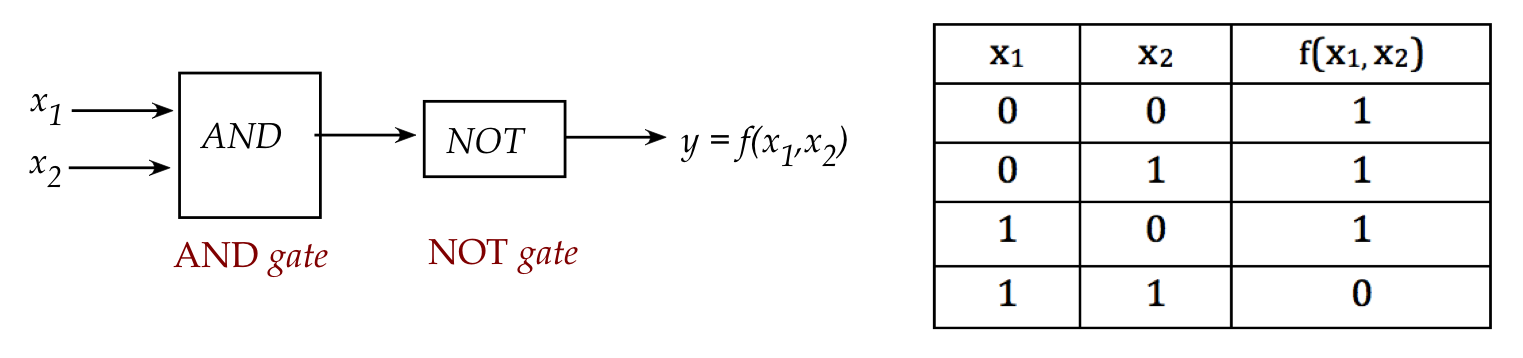
\includegraphics[width=5in]{notes/figs/n03/13_circuit3.png}
    \caption{AND NOT Electronic Circuitry Truth Table}
    \label{fig:13_AND_NOT_electronic_circuitry_truthtable}
\end{figure}

\begin{figure}
    \centering
    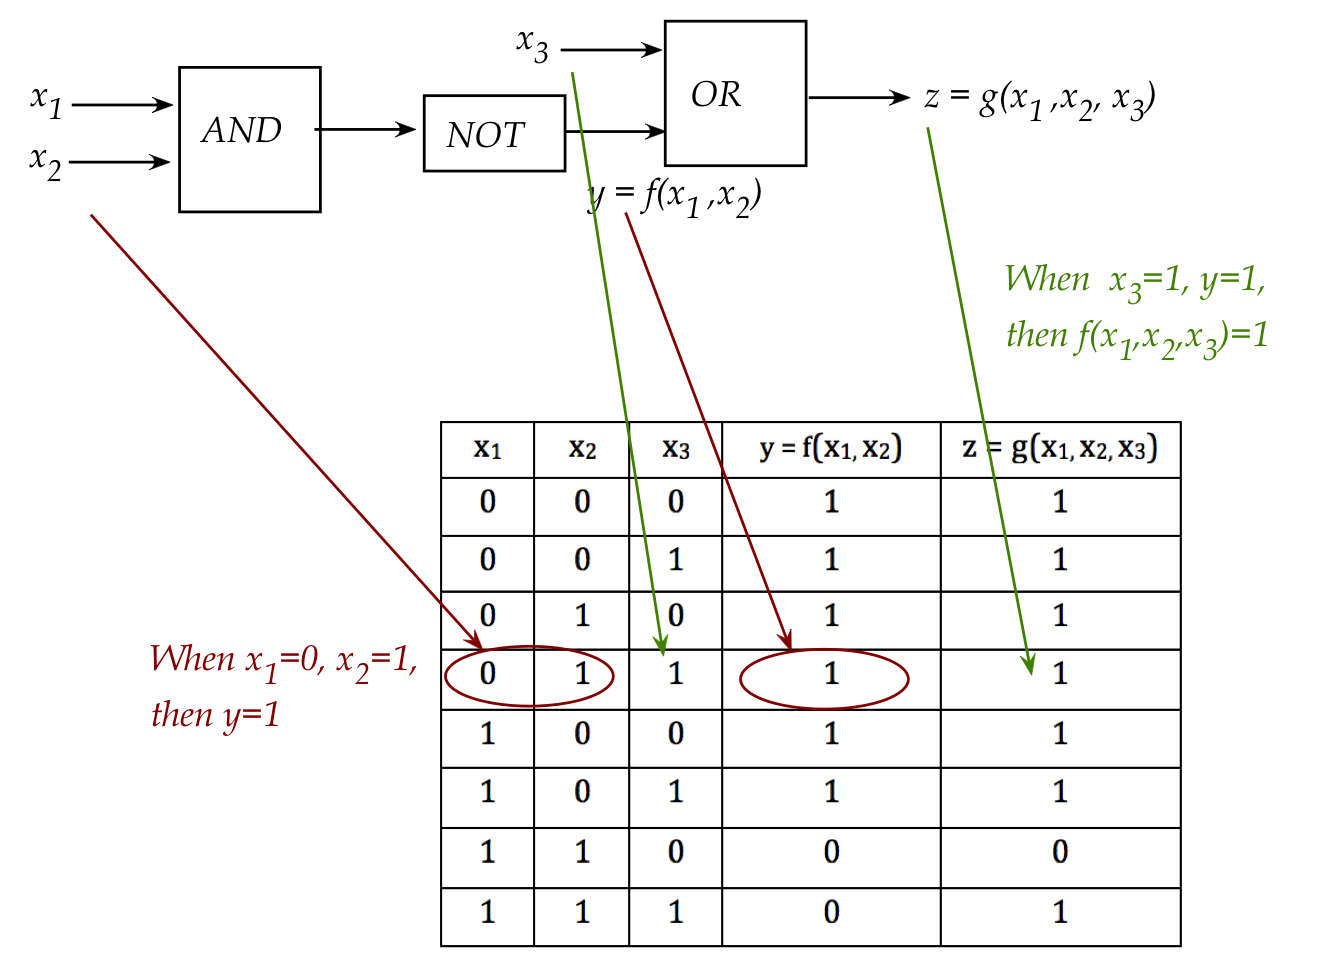
\includegraphics[width=5in]{notes/figs/n03/14_circuit4.png}
    \caption{AND NOT OR Electronic Circuitry}
    \label{fig:14_AND_NOT_OR_electronic_circuitry}
\end{figure}

Let's build a more useful circuit in steps: Suppose variables $x$ and $y$ represent two bits, and that we want to add them as shown in Figure \ref{fig:15_S_C_truthtable}. Notice: An addition of two bits produces two outputs: the sum and a carry (which will be used for positional addition later). What if there was a carry coming in? We'll worry about that shortly. The carry output is simply $x \wedge y$, which we shorten to $x y$. The sum output is $x^{\prime} y+x y^{\prime}$. Let's put this all together in a circuit for Figure \ref{fig16:half_adder}. Notice: We can branch off wires and route them to other gates. The circuit produces both the carry and sum outputs separately. We can use a half-adder box to represent the big circuit. This is called a half-adder because it does not account for a carry value that comes in from the previous bit in a number. Next, we'll use two half-adders to make a full. Suppose we want to add two 4-bit numbers in Figure \ref{fig17:4_bit_add}. Except for the very first pair of bits (one from each number, $x_{0}, y_{0}$, all others must account for any carry value that comes from the previous bit addition. The addition goes bit by bit going right to left, as we would do by hand. What we need is the circuit in Figure \ref{fig18:full_adder}. Note: We've drawn this up going down as opposed to left-to-right.We haven't said where the numbers are stored and how those bits are placed on the $x_{i}, y_{i}$ wires. One way to build a full adder is to write out the truth table and put the Boolean gates together. Alternatively, we can reason through using two half-adders as shown in Figure \ref{fig19:two_half_adders}. We'll re-draw the figure from earlier to go left-to-right, which is often the drawing convention used in quantum circuits as seen in Figure \ref{fig20:re-draw}. Finally, Figure \ref{fig21:condensed} is the condensed version treating the whole circuit as a building block. This approach of building progressively higher levels blocks is essential to managing the complexity of real systems, and for our own understanding of how stuff works.

\begin{figure}
    \centering
    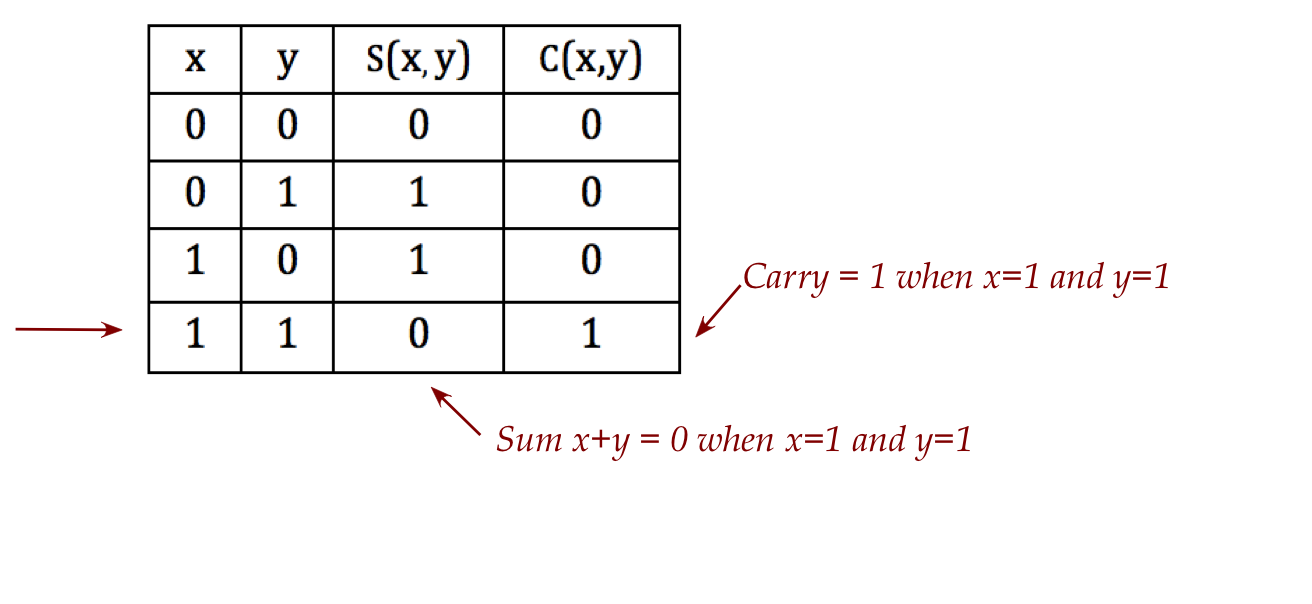
\includegraphics[width=5in]{notes/figs/n03/15_adder1.png}
    \caption{S C Truth Table}
    \label{fig:15_S_C_truthtable}
\end{figure}

\begin{figure}
    \centering
    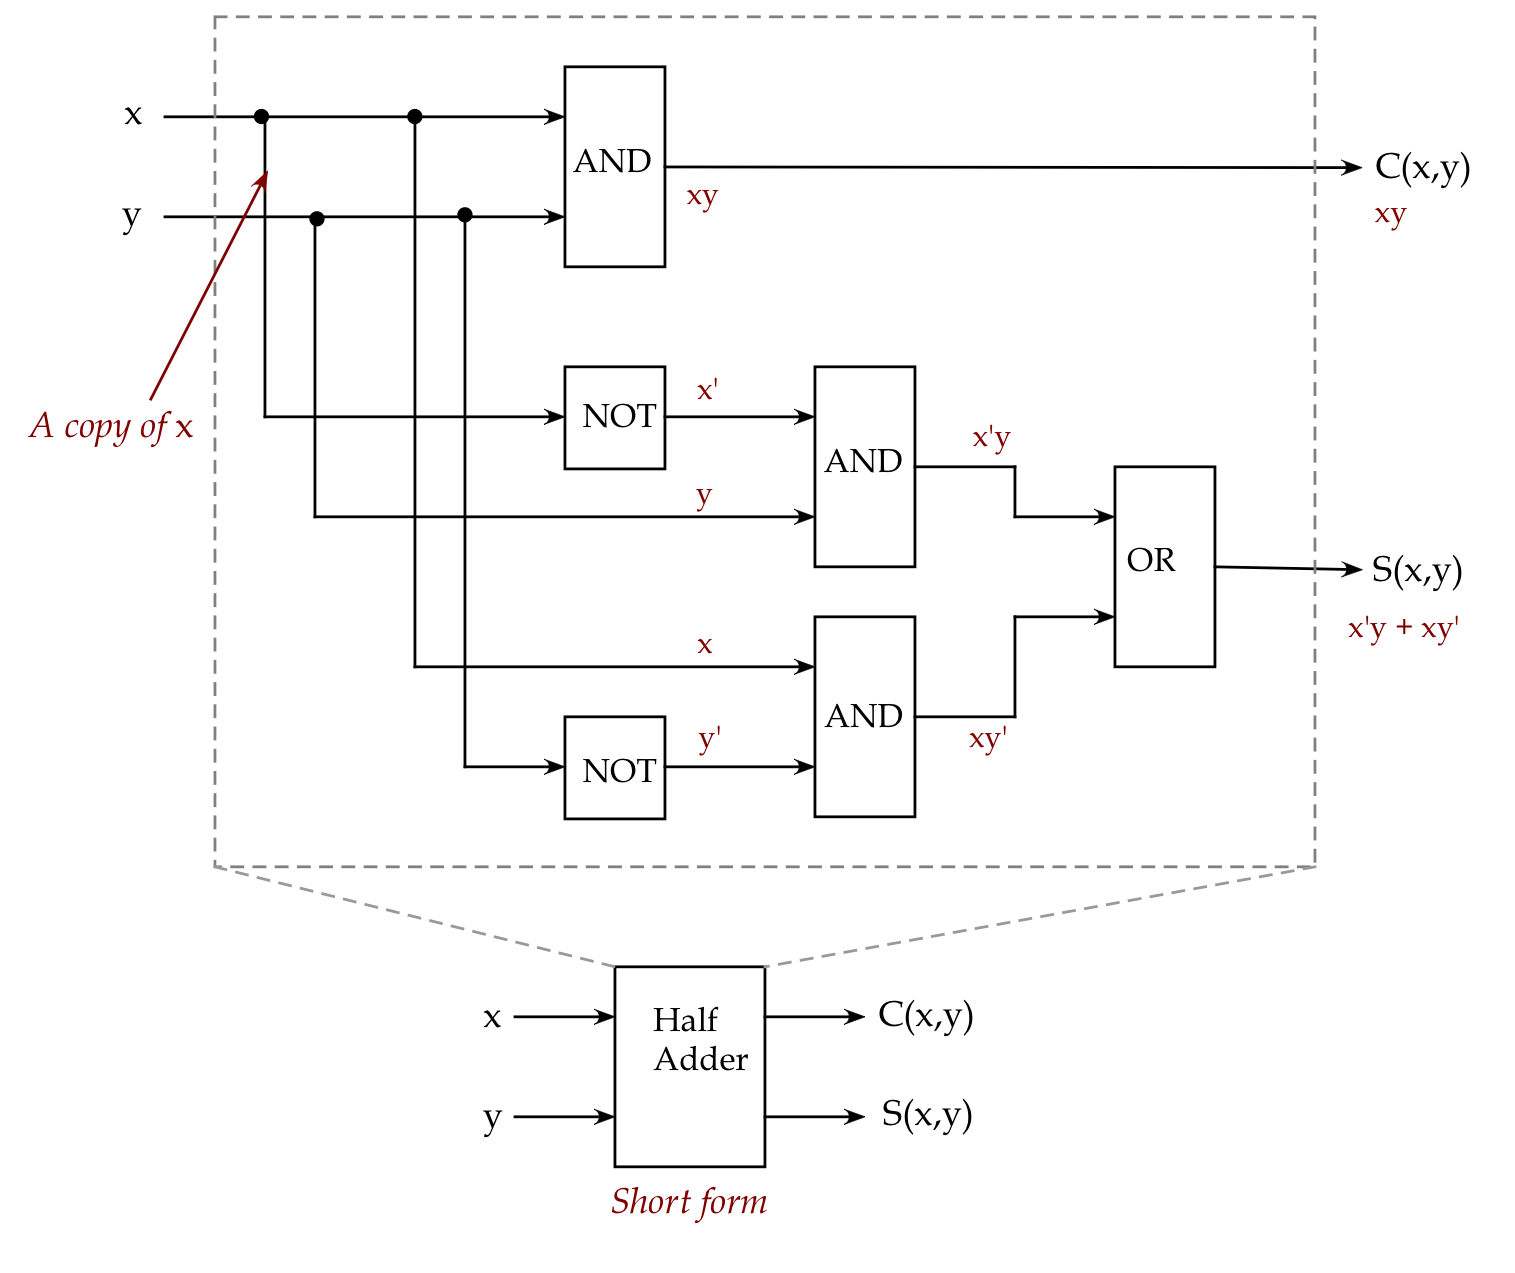
\includegraphics[width=5in]{notes/figs/n03/16_adder2.png}
    \caption{Half Adder}
    \label{fig16:half_adder}
\end{figure}

\begin{figure}
    \centering
    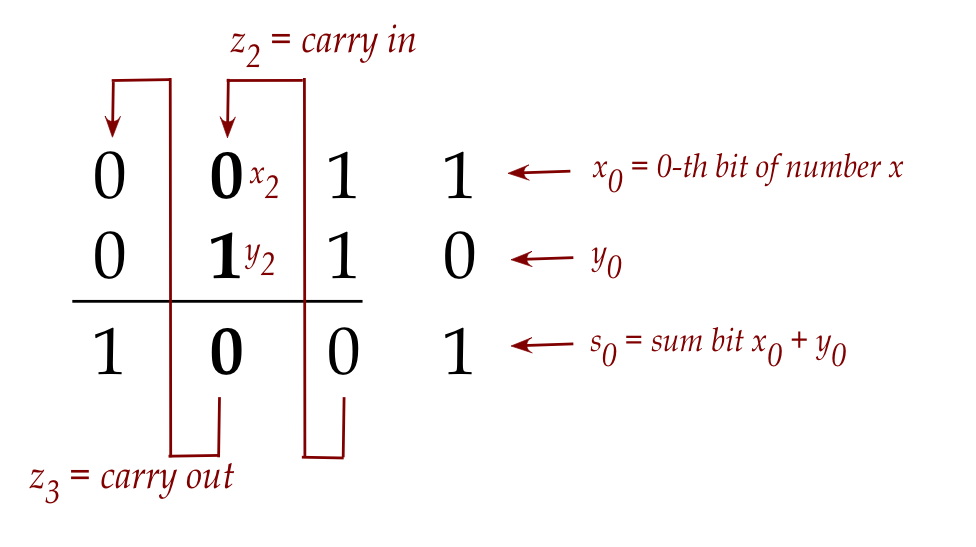
\includegraphics[width=5in]{notes/figs/n03/17_adder3.png}
    \caption{4 Bit Add}
    \label{fig17:4_bit_add}
\end{figure}

\begin{figure}
    \centering
    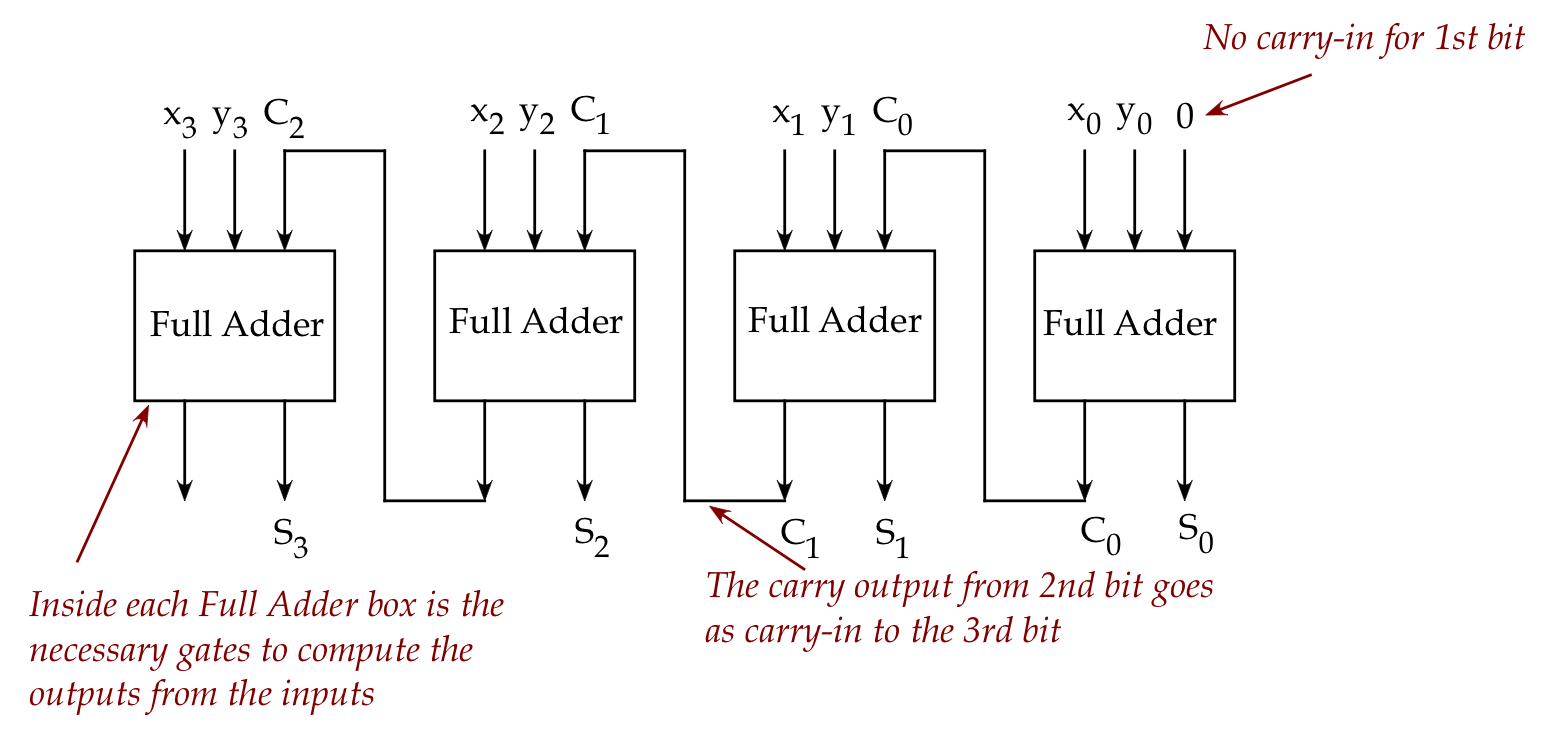
\includegraphics[width=5in]{notes/figs/n03/18_adder4.png}
    \caption{Full Adder}
    \label{fig18:full_adder}
\end{figure}

\begin{figure}
    \centering
    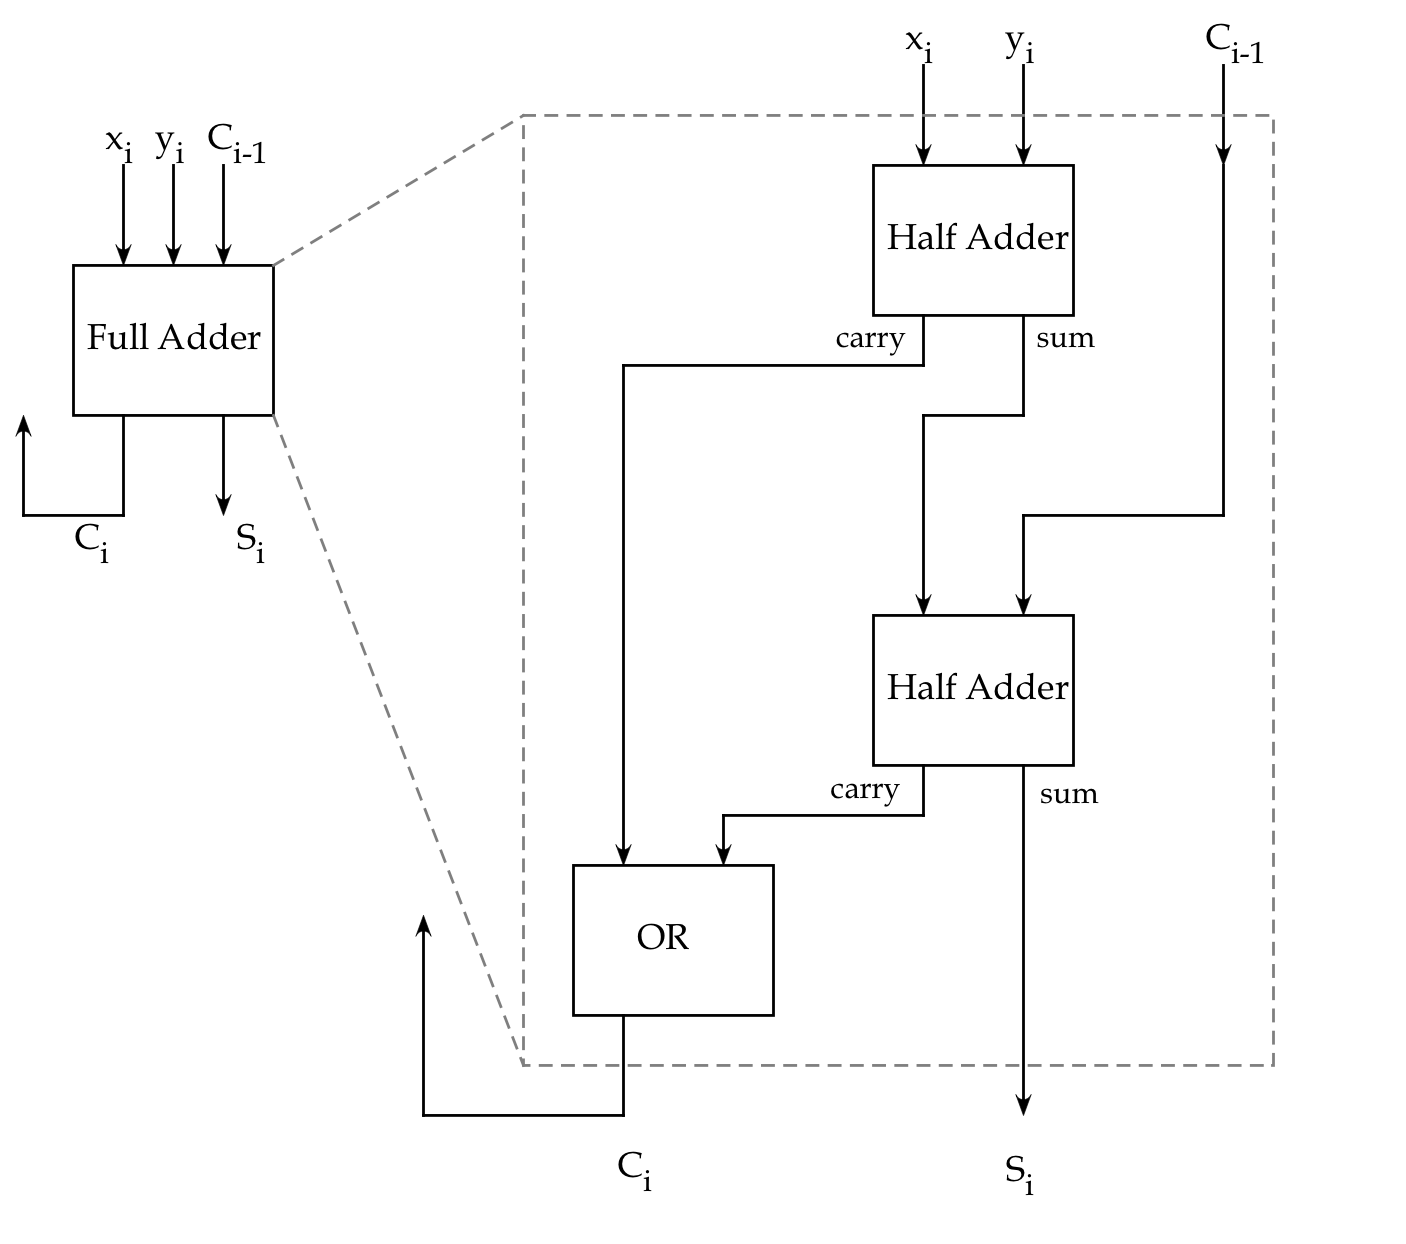
\includegraphics[width=5in]{notes/figs/n03/19_adder5.png}
    \caption{Two Half Adders}
    \label{fig19:two_half_adders}
\end{figure}

\begin{figure}
    \centering
    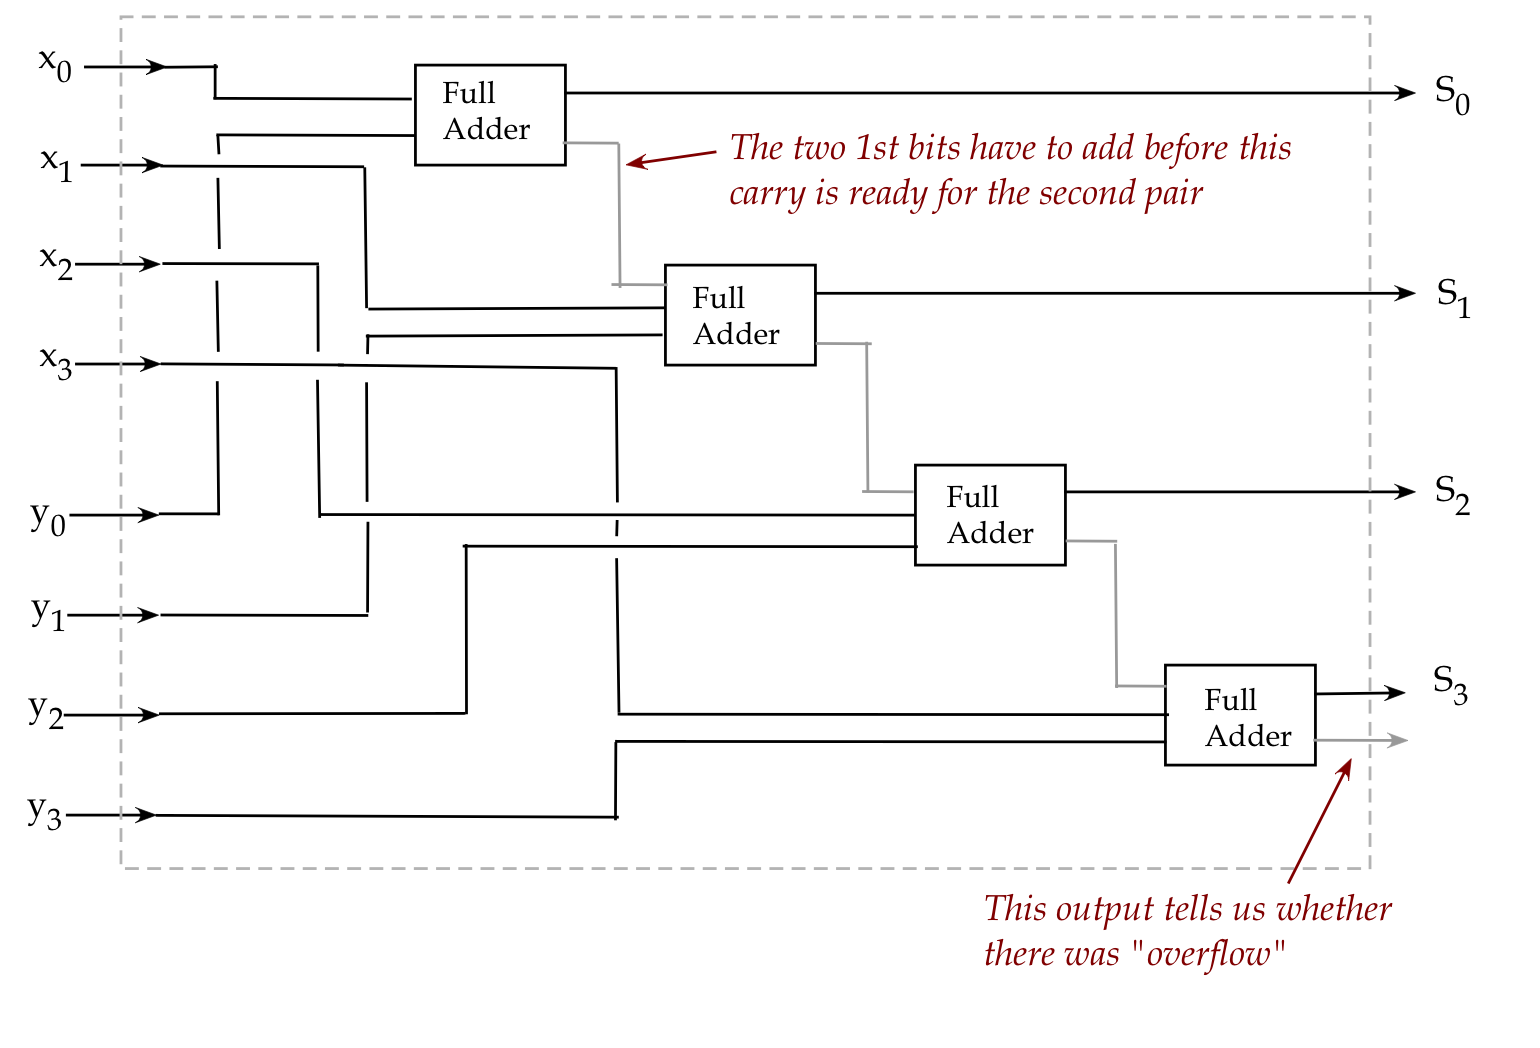
\includegraphics[width=5in]{notes/figs/n03/20_adder6.png}
    \caption{re-draw}
    \label{fig20:re-draw}
\end{figure}

\begin{figure}
    \centering
    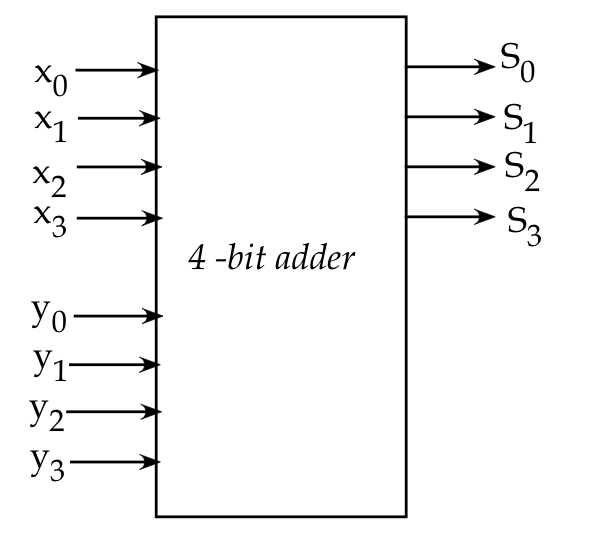
\includegraphics[width=3in]{notes/figs/n03/21_adder7.png}
    \caption{condensed}
    \label{fig21:condensed}
\end{figure}

\subsection{Registers and memory}

In all the circuits we've seen so far, we haven't mentioned where the inputs come from or where the output "goes". In the 4 -bit adder circuit above, for example, it's assumed that the inputs "arrive" at the input wires together. Then, the particular values (0's and 1') flow through the circuit, achieving the desired function. A little later, the output wires carry the resulting 0 's and 1 's that constitute the output as shown in Figure \ref{fig22:4-bit_adder}. All of the "action" in the circuit is fleeting and it happens very quickly. Clearly, to be of any use, we need to "hold" the results long enough for future calculations or for human interaction. One element of storage is a register, which is an array of 1-bit storage devices as shown in Figure \ref{fig23:4-bit_adder_with_register}. Each register can hold its value indefinitely (as long as there's power). When desired, the input registers can be told to send their values to the adder, which produces the output. The new added output replaces whatever was already there in the output register. Registers are typically named like R1, R2 etc. How do numbers get into the input registers to begin with? \\

\begin{figure}
    \centering
    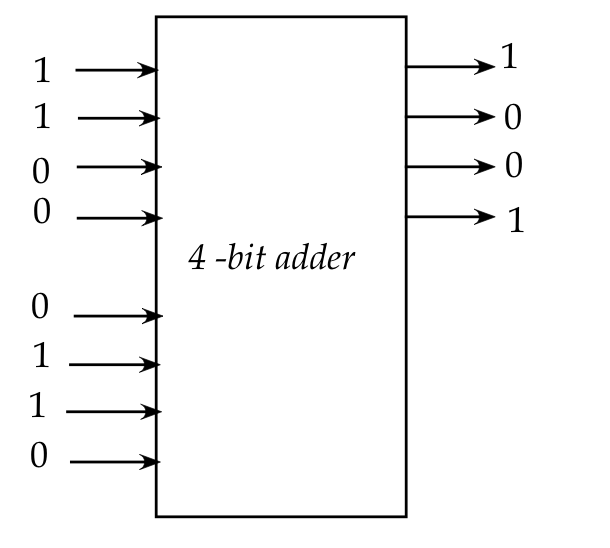
\includegraphics[width=3in]{notes/figs/n03/22_adder8.png}
    \caption{4-bit adder}
    \label{fig22:4-bit_adder}
\end{figure}

\begin{figure}
    \centering
    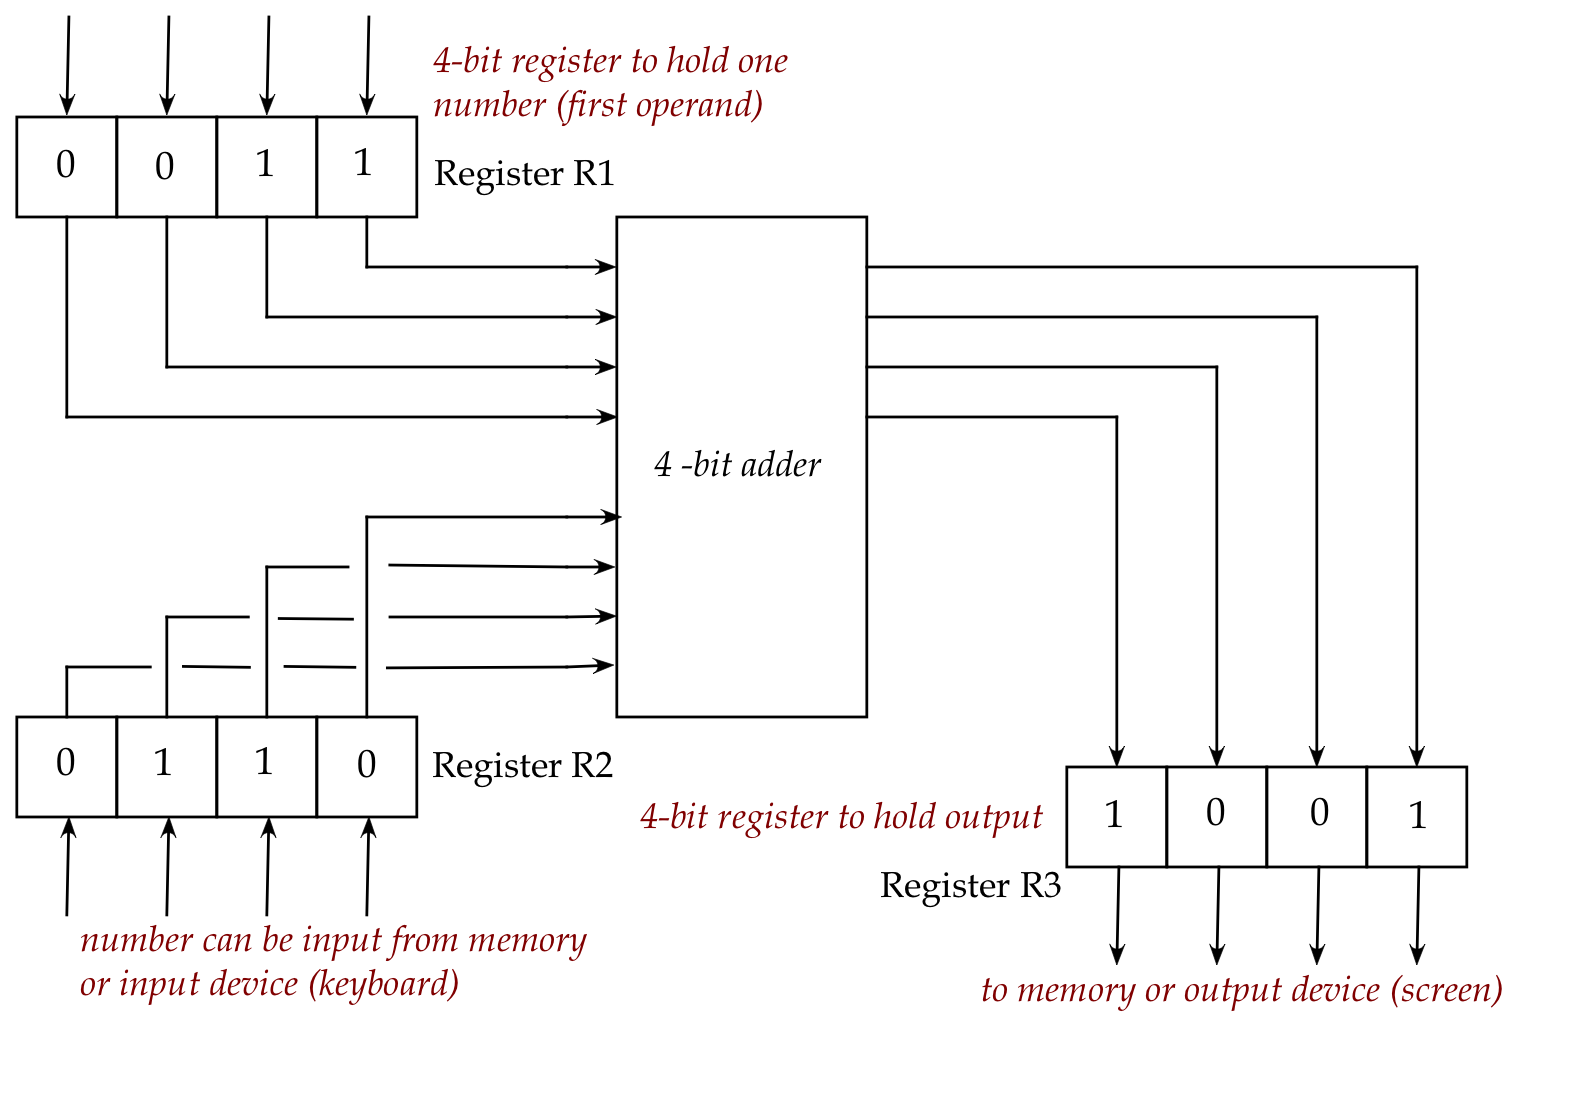
\includegraphics[width=4in]{notes/figs/n03/23_adder9.png}
    \caption{4-bit Adder with Register}
    \label{fig23:4-bit_adder_with_register}
\end{figure}

Computing devices need more than registers to store data: This is accomplished with random access memory, also called RAM or main memory. By memory, we mean a computer's main memory as opposed to hard disk or removable media like drive's. You can think of a memory chip as box with the following functions: Reading: You give it a memory address; it gives you the contents of that memory address, for Writing: You give it a memory-address and a value, and it stores the value in that location as shown in Figure \ref{fig24:read_write_memory}. A conceptual way to think of memory is: a hotel reception desk with mailboxes. When you want to get (read) something: you provide your mailbox number (memory-address) and the concierge gives you the contents. When you want to put (store) something: you provide the contents and the mailbox number (address), and the concierge stuffs it in. Conceptually, it helps to think of memory as a long collection of numbered locations as shown in Figure \ref{fig26:memory_numbered_locations}. The numbers are the addresses.

\begin{figure}
    \centering
    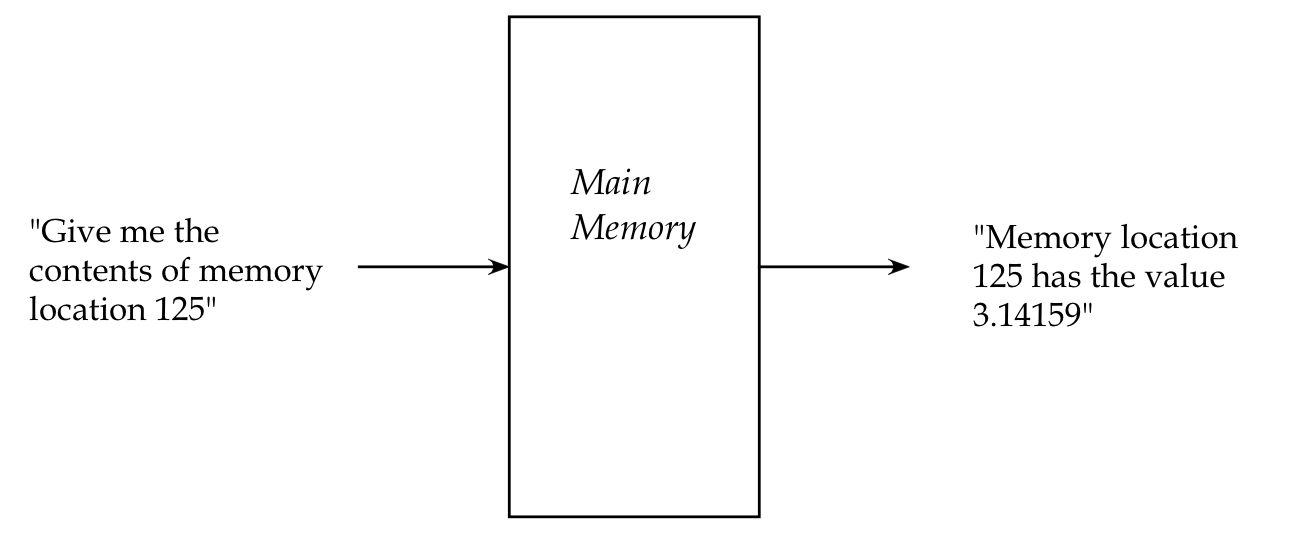
\includegraphics[width=3in]{notes/figs/n03/24_memory1.png}
    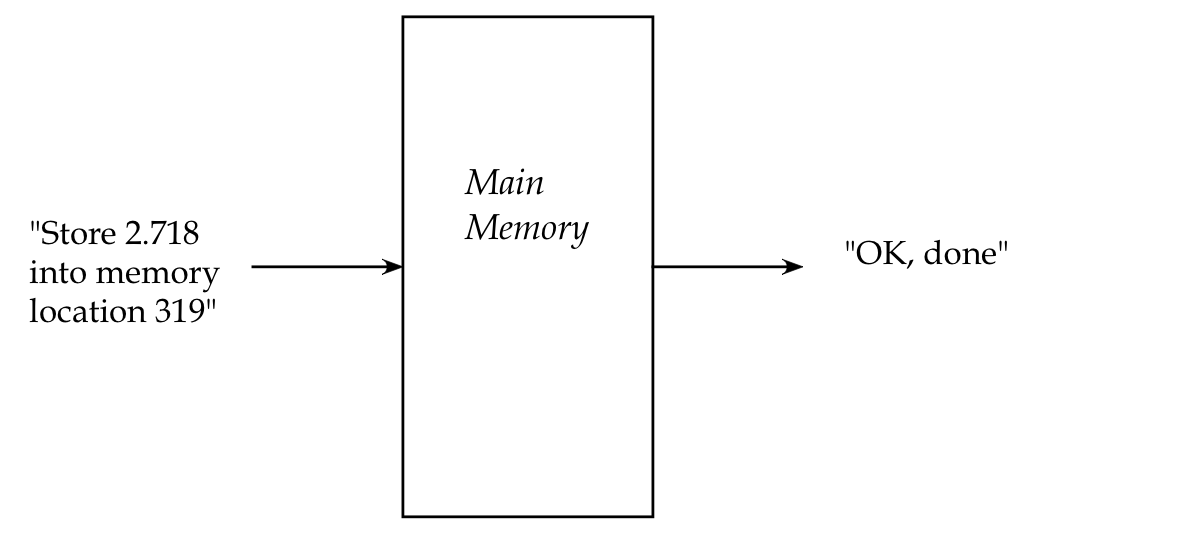
\includegraphics[width=3in]{notes/figs/n03/25_memory2.png}
    \caption{Reading and Writing to Main Memory}
    \label{fig24:read_write_memory}
\end{figure}

\begin{figure}
    \centering
    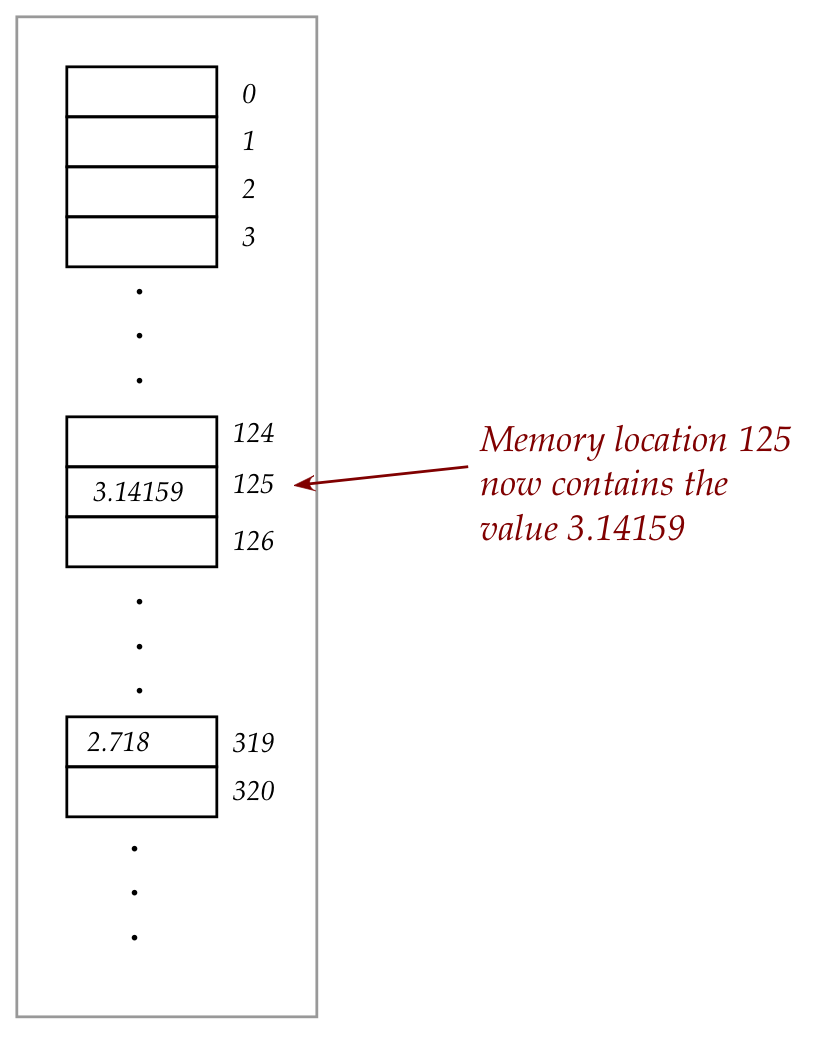
\includegraphics[width=3in]{notes/figs/n03/26_memory3.png}
    \caption{Memory numbered locations}
    \label{fig26:memory_numbered_locations}
\end{figure}

\subsection{The Von Neumann architecture}

Consider for a moment the most basic calculator that can perform only addition, subtraction, multiplication and division: The components of such a calculator are shown in Figure \ref{fig27:calculator_components}. A main register that one sees when typing in numbers. A secondary register (not seen) to hold the most recent result. A bunch of circuitry to perform the arithmetic operations. What's important to note: the process of calculation is driven by the human who organizes the calculations. Consider calculating $2 *((3+6)-5)$. If one were to instruct another person to use the calculator, the instructions could be something like:

\begin{enumerate}
    \item Load 3
    \item Load 6
    \item Add
    \item Load 5
    \item Subtract
    \item Load 2
    \item Multiply
\end{enumerate}

\begin{figure}
    \centering
    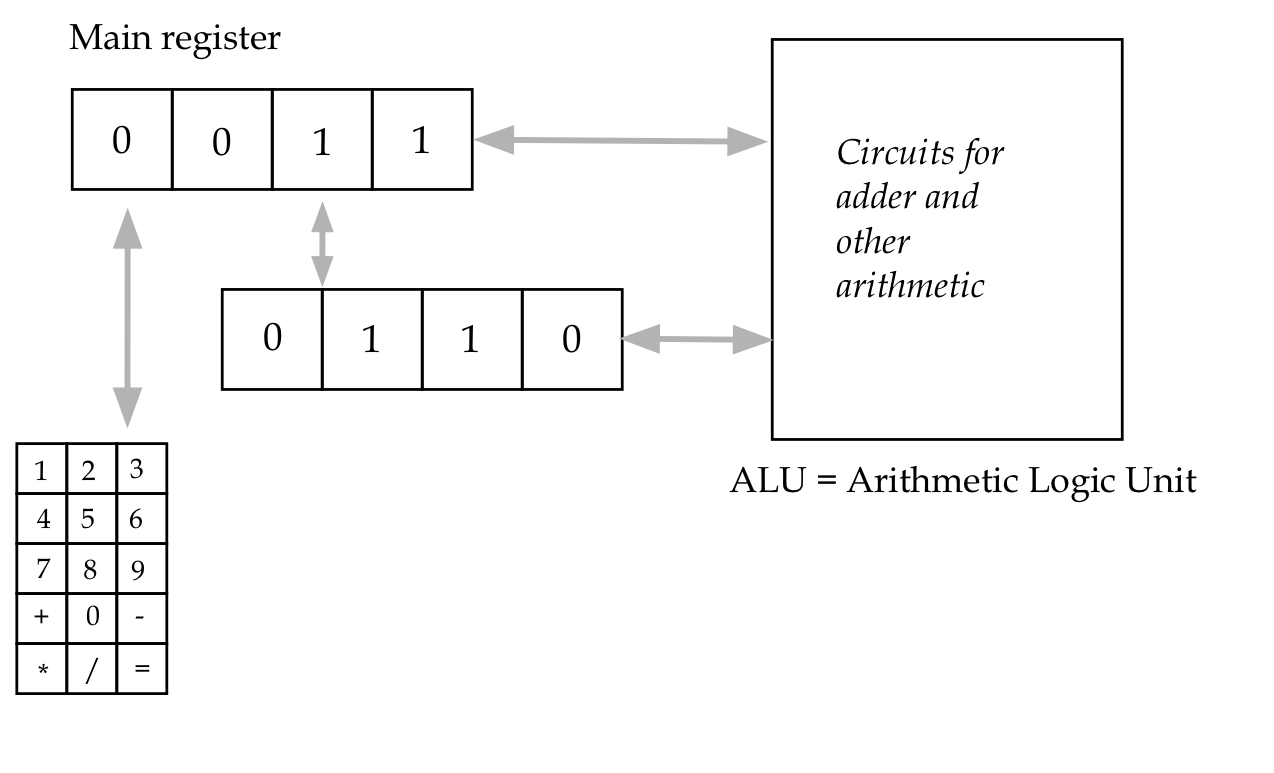
\includegraphics[width=3in]{notes/figs/n03/27_calculator.png}
    \caption{Calculator Components}
    \label{fig27:calculator_components}
\end{figure}

Think of the list of 7 instructions above as a program that achieves the task of "calculating $2^{*}((3+6)-5)^{\prime \prime}$. In the hardware of a computer, as opposed to a calculator, it is precisely such a program that is executed step-by-step. The same program in a computer: If no human orchestration is to occur, the data (the numbers $2,3,5,6$ ) need to be in memory. Suppose that the numbers are stored from location 0 onwards. The program (of instructions) that carry out the calculation would look like:

\begin{enumerate}
    \item Load from location 0
    \item Load from location 1
    \item Add
    \item Load from location 2
    \item Subtract
    \item Load from location 3
    \item Multiply
    \item Store in location 8
\end{enumerate}

The Von Neumann architecture shown in Figure \ref{fig28:von_naumann_architecture}: If a program is to be executed quickly, the instructions need to be in electronic form and stored somewhere. The (so-called) Von Neumann architecture solves this problem by re-using the bit-patterns in memory to encode such instructions. Thus, a particular bit pattern like 1101 if interpreted as data will be the number $13$. When interpreted as an instruction, it means "load". (The hardware designers decide these interpretations.) Then, what remains to be done is an 'orchestrating' unit that directs the sequence of actions. Note: The data and instructions are both stored in memory, typically in separate parts. The controller knows how to interpret the bit patterns that represent instructions. The controller also knows how to sequence the instructions. What's interesting is that the controller itself is built out of the same units (gates, registers) so that everything runs fast.

\begin{figure}
    \centering
    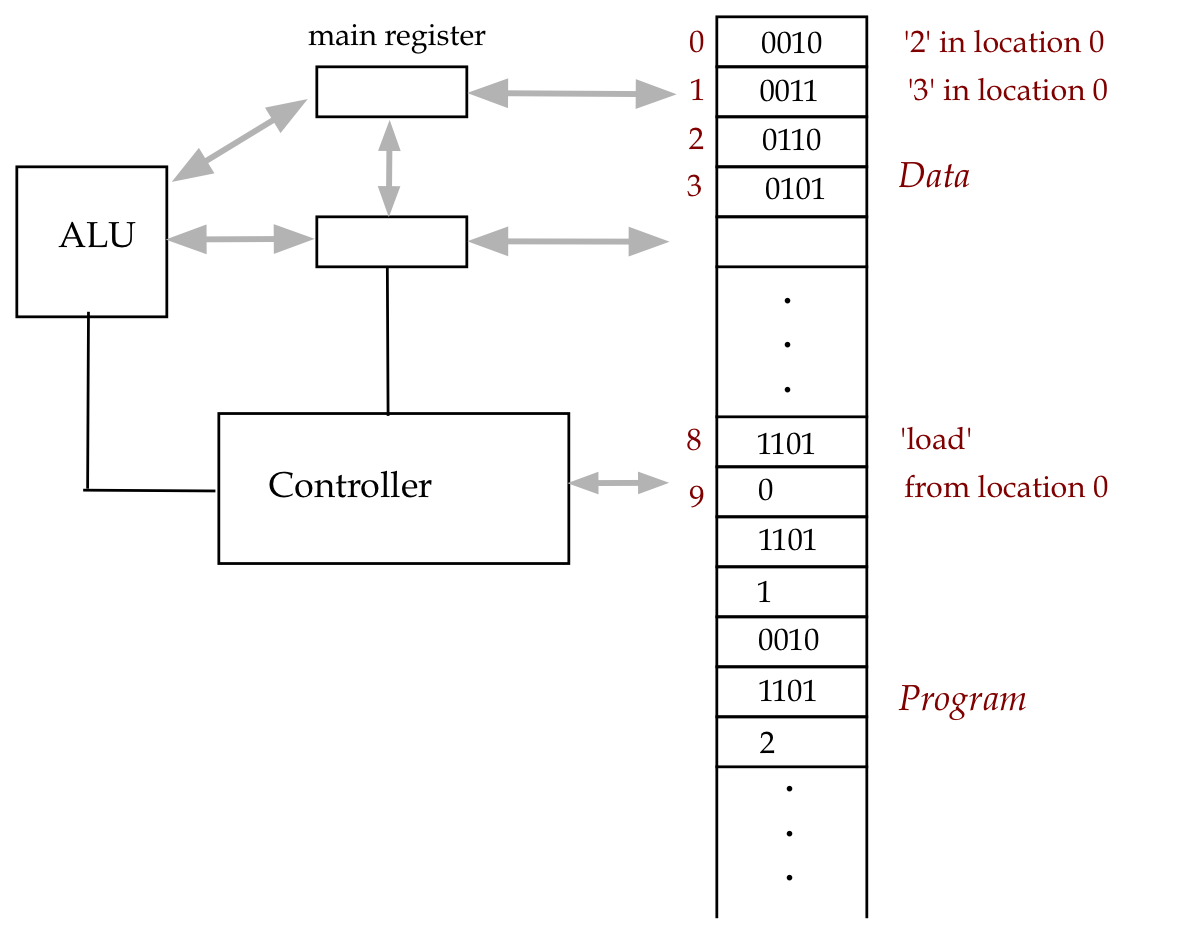
\includegraphics[width=4in]{notes/figs/n03/28_program.png}
    \caption{Von Neumann Architecture}
    \label{fig28:von_naumann_architecture}
\end{figure}

\subsection{Networks and security}

Let's examine networks in a simplified way: A laptop wirelessly connects to a wireless access point. This connects to a router (which may be combined with the access point at home). The router connects to a larger router operated by telecom company or larger router in an organization. The larger routers then connects to even larger routers that form the backbone of the internet. Each particular connection can be thought of as providing a way to transmit bits from one side to another as shown in Figure \ref{fig29:transmit_bits}.We're using a line conceptually to mean either an actual wire or wireless. At any one moment, one side transmits while the other receives. The above example shows how the bits 1011 might look like going across. Our focus is going to be security as shown in Figure \ref{fig30:transmit_security}: In the typical style of security presentations, one person A (for Alice) transmits something to person B (Bob), while person E (Eve) listens in. What do Alice and Bob want? Confidentiality: Eve shouldn't be able to understand, even if she successfully copied the bits. Integrity: Eve should not be able to manipulate the bits Bob receives, or at least Bob should know if this happened. Authenticity. Eve should not be able to masquerade as Alice to Bob, or the other way around. Availability: If Eve simply blocks transmission, Alice and Bob should know. Thus, measure to improve security need to address such concerns.
Typically, one uses encryption to protect confidentiality.
To protect integrity: The encrypted message should itself contain something (a digest) such that any tampering is detected. The message should contain something to verify that it is Alice that indeed sent the message (to catch Eve if she masquerades as Alice). To protect availability, Alice and Bob can arrange to send pre-determined bits at certain intervals. There is a whole world of potential attacks and measures to defend. We won't be able to go into all the details. And there's a whole world of encryption mathematics and techniques, some of which uses integer factoring as a foundation.\\

\begin{figure}
    \centering
    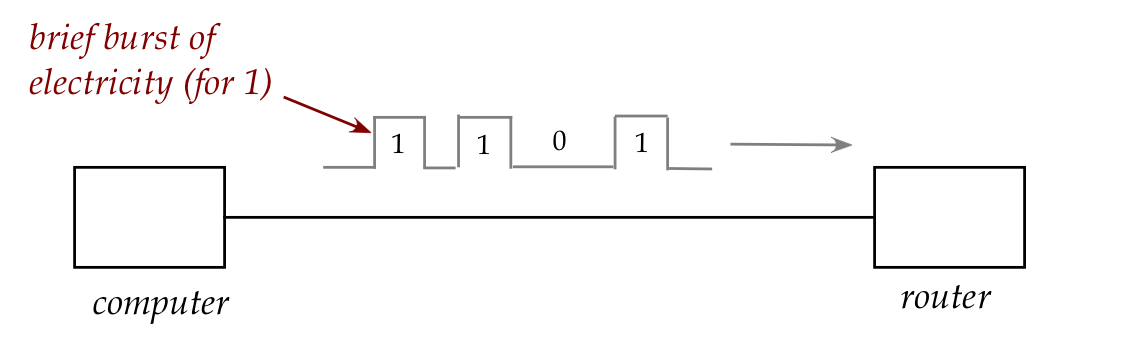
\includegraphics[width=4in]{notes/figs/n03/29_network1.png}
    \caption{Transmit bits}
    \label{fig29:transmit_bits}
\end{figure}

\begin{figure}
    \centering
    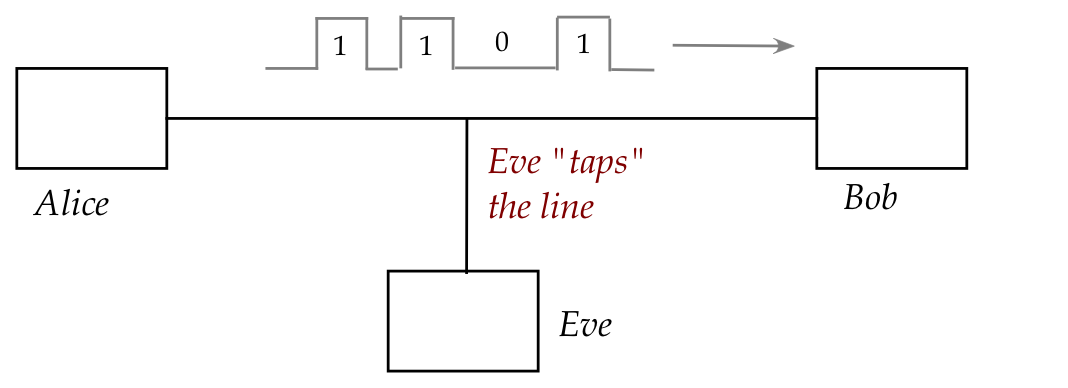
\includegraphics[width=4in]{notes/figs/n03/30_network2.png}
    \caption{Transmit Security}
    \label{fig30:transmit_security}
\end{figure}

Quantum computing focuses on two aspects of security: Using a quantum computer to break encryption: This is the famous Shor's Algorithm for factoring integers. Our goal will be to understand how this works. Using transmission of quantum bits to provide security: We will show that quantum bits have unusual properties that enable strong security properties. For example, if Eve even "looks" at bits going by, Alice and Bob will know.

\subsection{The state of computing today}

First, a software/algorithms perspective: The past few decades have seen much progress in: Fast algorithms for many computational problems. Clever solutions to thorny security problems. Software infrastructure and tools that exploit inexpensive hardware to scale solutions. But at the same time, there are stubbornly hard problems resistant to algorithmic development: Many of these are the so-called combinatorial optimization problems. Examples include: scheduling, routing, network design, and a host of such optimization problems. There's also theory that remains to be solved: Example: nobody has proved that factorization is hard, nor is there a fast algorithm. A hardware perspective: Each year, more and more gates get packed into the same space, allowing a continuing miniaturization trend, sometimes called Moore's Law. But miniaturization is now creeping up on limits imposed by physics: When you get down to the size of atoms, the laws of physics that typically apply at higher scales are now dominated by quantum physics. This means quantum effects apply, whether desirable (as in the case of quantum computing) or not. Another issue is heat: the more you pack into the same space, the more heat you dissipate per unit area, and the harder it is to cool. The other trend is massive parallelism (using many processors for a single computation) but that comes with caveats too: It is hard to write programs for parallel machines. Some problems are resistant to parallelism. Parallelism can be expensive if most of the processors are idle because parallelism cannot be extracted. Yet another trend is hardware specialization: The idea here is to design specialized hardware optimized for particular tasks. The most prominent example is GPUs for high-speed graphics. A newer example is: hardware for machine-learning. It's hard to say where these trends will take us. But this is precisely why it's an interesting time: the nexus of quantum hardware, parallelism and specialization points to a exciting future!

\end{document}